\chapter{Matter and Energy}

\section{Matter and Energy}
% authors note: verified against AP Phys C 19th edition chapter 13
The universe is made of matter and energy. Current models posit that the universe
is approximately 68\% dark energy\index{dark energy}, 27\% dark matter\index{dark matter}, and 5\% ordinary matter.
Everything you can see and touch is part of the small part of the universe made 
of ordinary matter. Most science deals with ordinary matter and its interactions; 
highly trained theoretical physicists are currently debating the nature and 
effects of dark matter and dark energy. 
\begin{wrapfigure}{r}{2.2in}
\noindent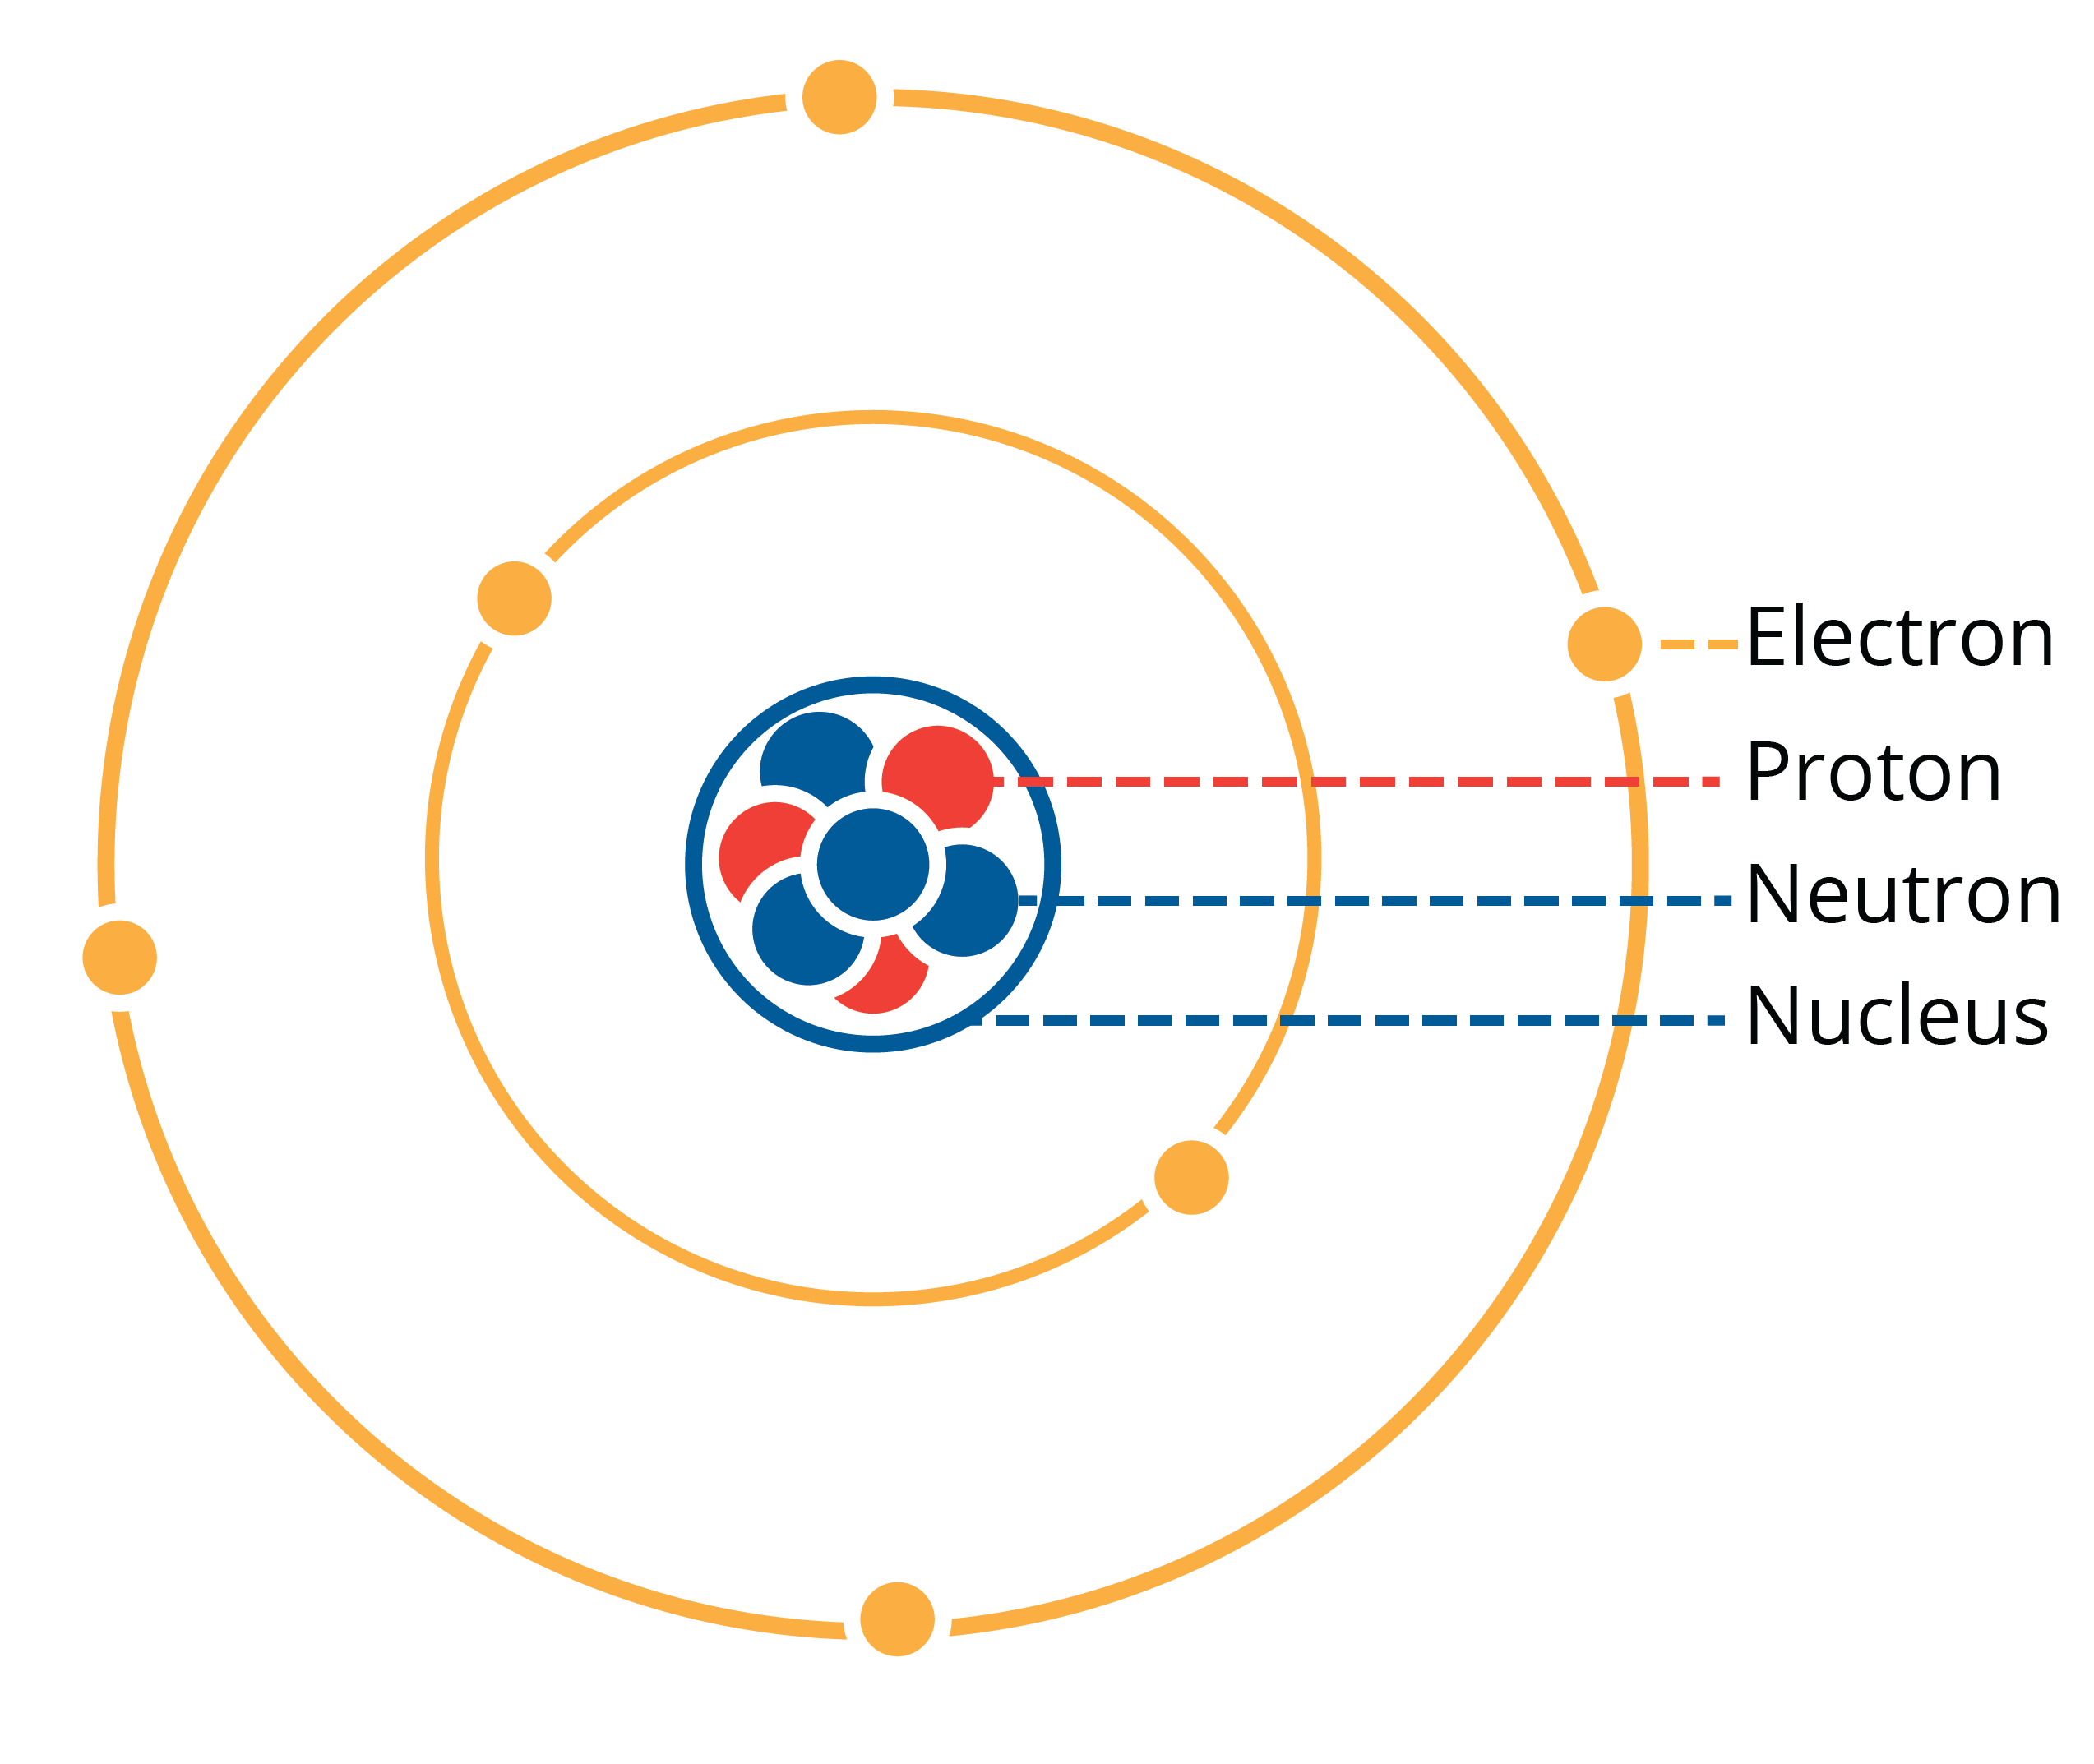
\includegraphics[width=2.5in]{atom1.png}
\caption{}
\label{fig:atom1}
\end{wrapfigure}

What is this ordinary matter made of? All things (including the air around you) 
are made of \textit{atoms}. Atoms are incredibly tiny --- there are more atoms in a drop 
of water than there are drops of water in all the oceans. Sizes like that are hard to picture. \href{https://htwins.net/scale2/}{The Scale of the Universe}, a website by Cary and Michael Huang, lets you zoom from galaxies down to quarks. Start at $10^{-15.5}$ meters to see protons and neutrons.

Every atom has a \textit{nucleus} that contains \textit{protons} and \textit{neutrons}. Orbiting around the
nucleus is a cloud of \textit{electrons}. However, the mass of the atom comes mainly from 
the protons and neutrons, since they are about 2000 times as massive as an 
electron! These three particles, protons, neutrons, and electrons, are called
\textit{subatomic particles}. (See figure \ref{fig:atom1}.)

Studies such as particle physics, nuclear physics, and astrophysics analyze how these particles interact. 

An atom is mostly empty space. If the nucleus were a marble in the middle of a football stadium, the electrons would be specks buzzing around the outer seats. What holds them there? The \textit{electromagnetic force}\index{electromagnetic force}: the positive protons attract the negative electrons.

Every charged particle surrounds itself with an \emph{electric field}\index{electromagnetic field}, and moving charges also make a \emph{magnetic field}. That is why an electric current, which is just electrons moving through a wire, can push a compass needle.

% this content is added in the charge chapter but leaving it here, commented out
% Each subatomic particle can have its own distinct electric charge. Particles of the same charge repel each other, and particles of different charge attract. Protons have \emph{positive charge}, while electrons have \emph{negative} \index{protons} 
\index{neutrons} \index{electrons} \index{subatomic particle}
% https://en.wikipedia.org/wiki/Electromagnetic_field info on em fields

\subsection{Atoms and Their Models}
\begin{wrapfigure}{l}{3in}
\vspace{-0.2in} % prevent fig on new page
\noindent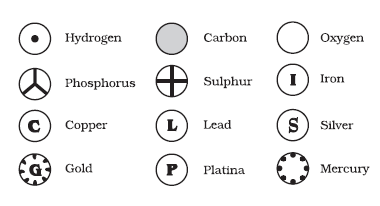
\includegraphics[width=2.5in, trim={0 0.5cm 0 0.5cm}, clip=true]{daltons_model.png}
\caption{}
\end{wrapfigure}

Our picture of the atom has changed a lot. Around 1800, John Dalton pictured atoms as tiny, solid, indivisible balls. Then in 1897, the British physicist J.J. Thomson discovered the electron: a light, negatively charged particle that can be pulled out of any atom. Atoms, it turned out, have parts.

In 1911, Ernest Rutherford fired tiny particles at a thin sheet of gold. Most went straight through, but a few bounced almost straight back, ``as if you fired a 15-inch shell at a piece of tissue paper and it came back and hit you,'' he said. The atom, he concluded, is mostly empty space, with its positive charge and almost all its mass packed into a tiny, dense \emph{nucleus}.
Subsequently, Niels Bohr explained the phenomena of spectral lines (we will discuss
this further in Sequence 2) by proposing that electrons
orbit at specific distances from the nucleus.

\begin{wrapfigure}{l}{2in}
\noindent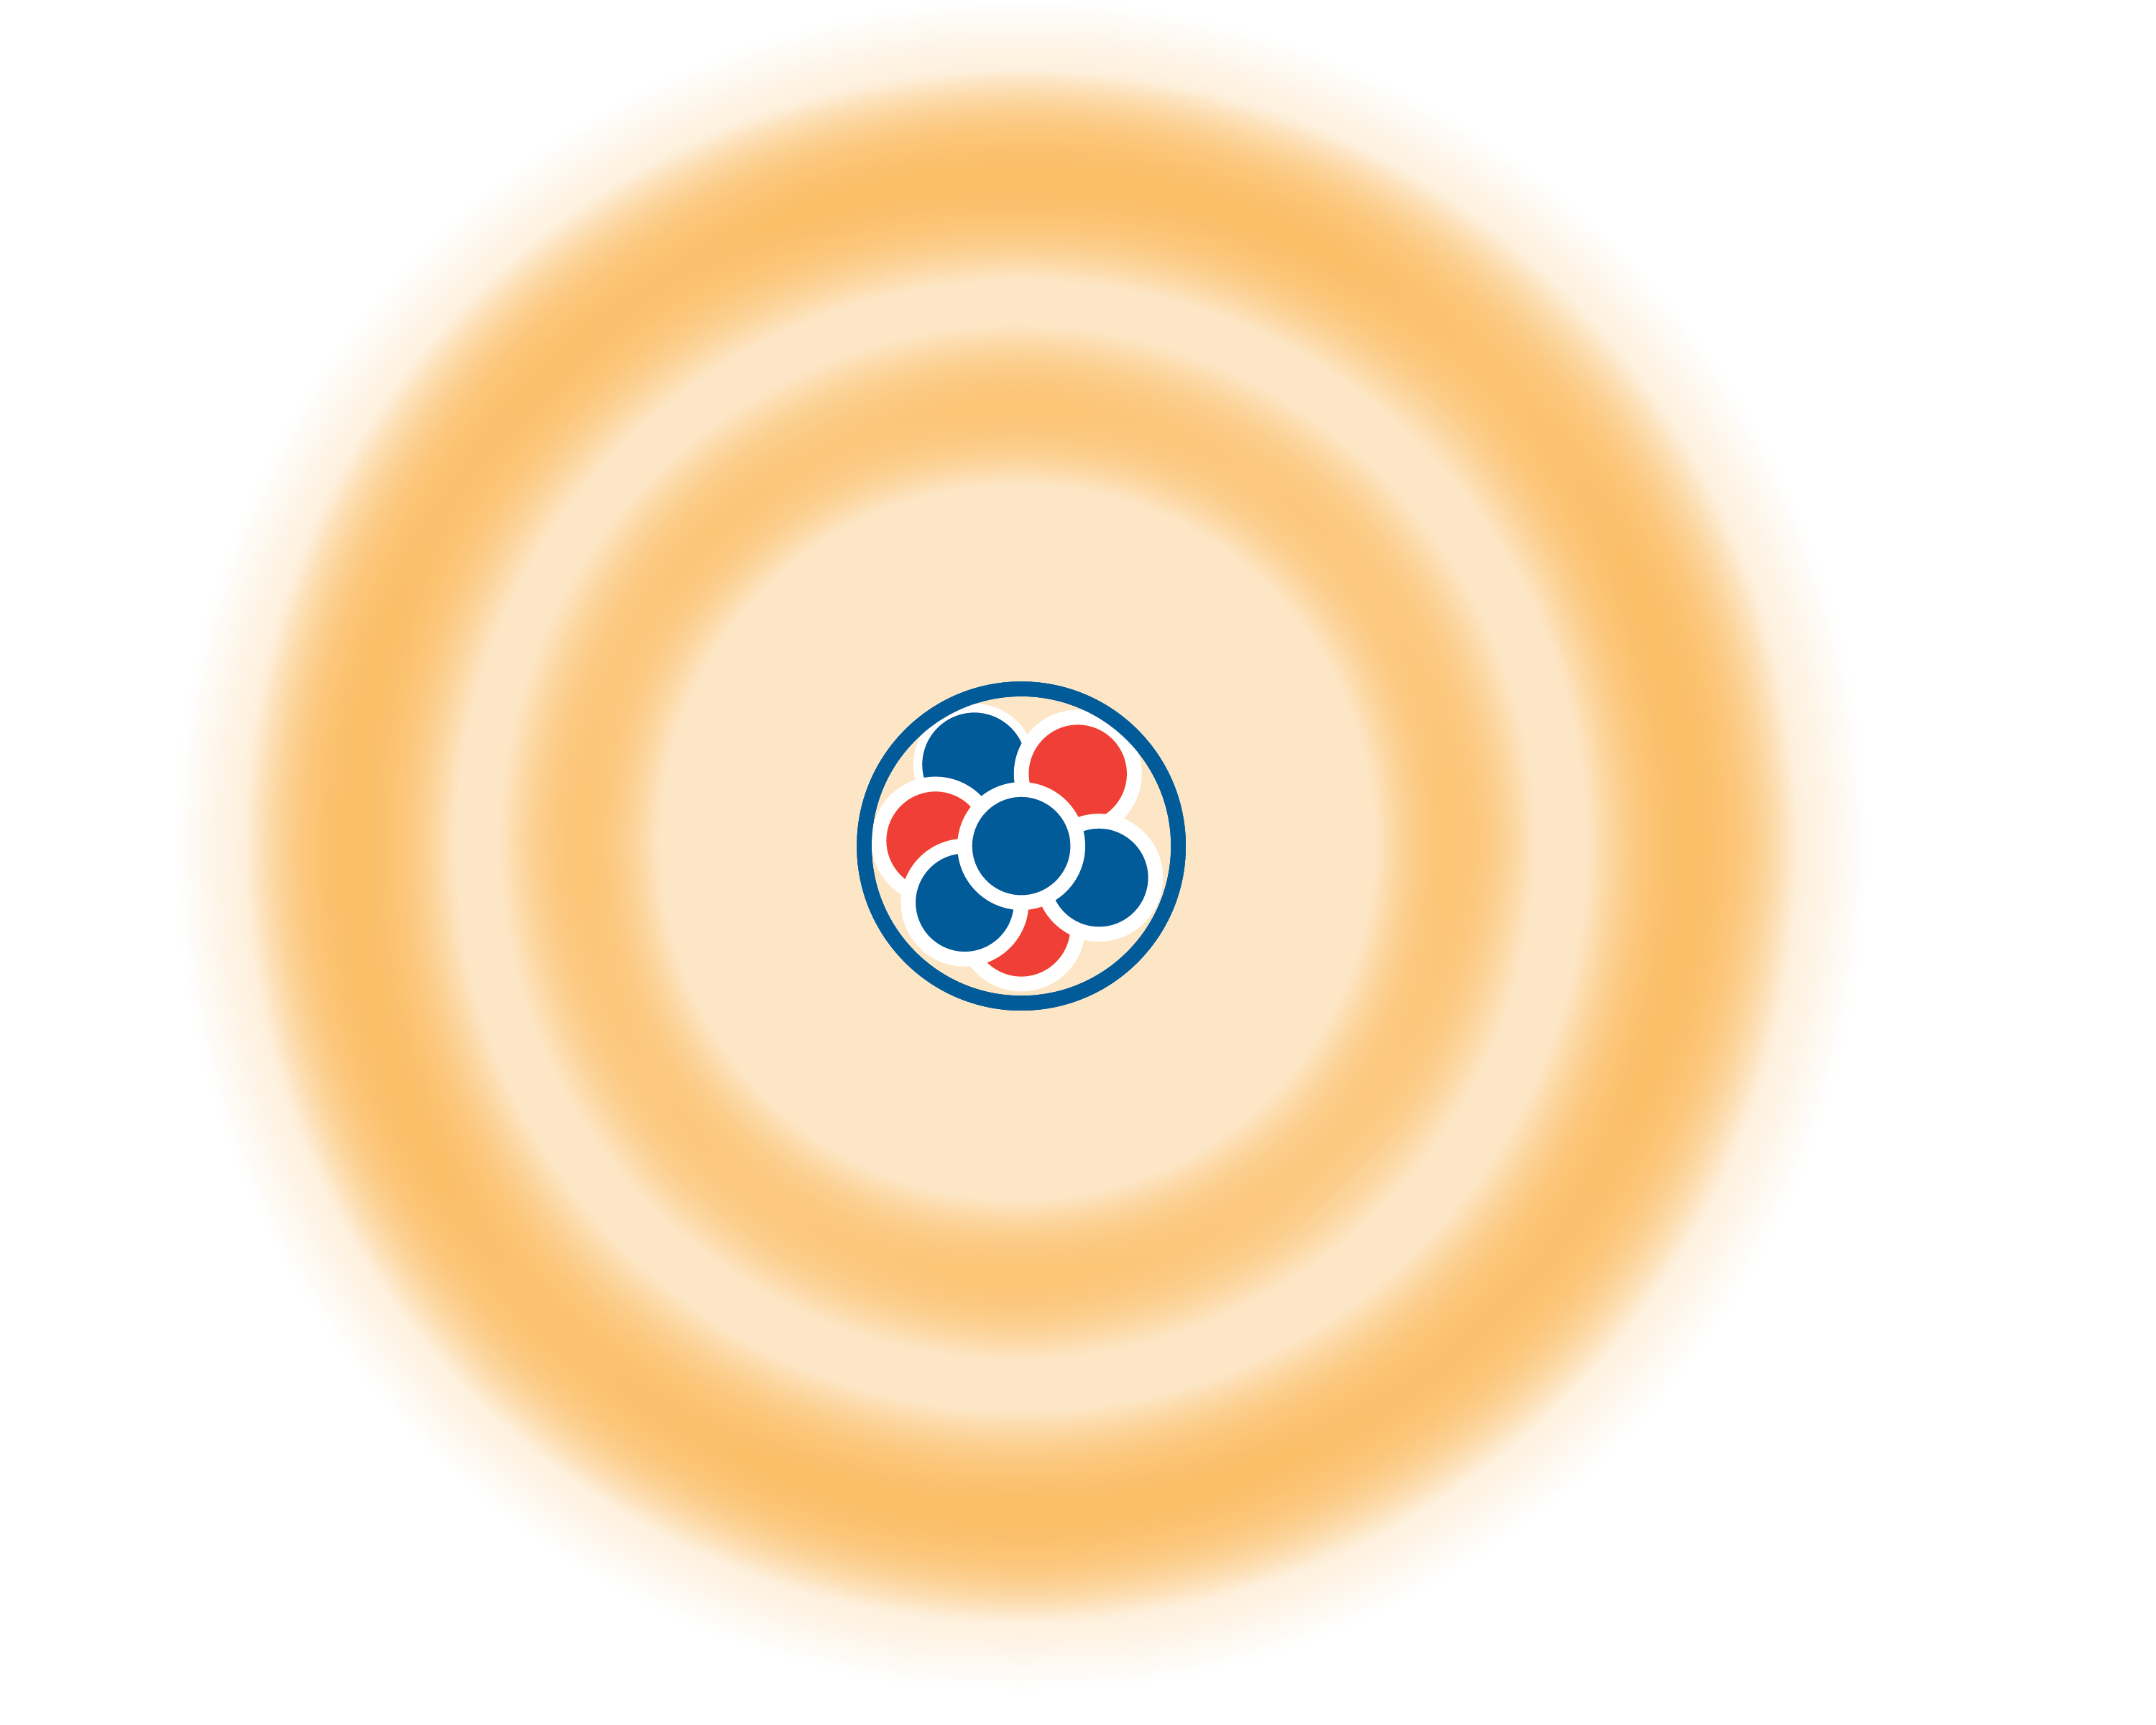
\includegraphics[width=2in]{atomCloud.png}
\caption{}
\label{fig:atomCloud}
\end{wrapfigure}

This is likely the model you are most familiar with seeing, and it is the one we
will use most often in this text. The first figure shown in this chapter is a Bohr
model: it shows the protons and neutrons in the nucleus, and models the electrons 
as moving in discrete orbits around the nucleus. 

However, the Bohr model is slightly inaccurate. While it is a convenient model for
thinking about atoms, in reality, electrons do not neatly orbit the nucleus.
Scientists do not know exactly where an electron will be in relation to the
nucleus, but they do know where it is most likely to be. They use a cloud that is
thicker in the center but fades out at the edges to represent an electron's
position (see figure \ref{fig:atomCloud}).  This cloud represents the probability
distribution of finding an electron in a particular region around the nucleus. The
figure is only in two dimensions, but the actual electron cloud is three-dimensional.
The shape of the cloud depends on the energy level of the electron, and different
energy levels have different shapes and sizes of clouds.

While the cloud model is more accurate, we will use the Bohr model as it
allows you to easily and quickly assess the number and arrangement of
electrons.


\subsubsection{Classifying Atoms}
\begin{wrapfigure}{r}{2.5in}
    \centering
    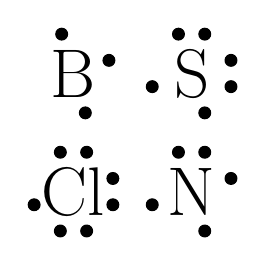
\begin{tikzpicture}
        \node[font=\Huge] at (-0.75,0) {B};
        \draw[fill=black] (-0.9, 0.5) circle (0.75mm);
        \draw[fill=black] (-0.3, 0.167) circle (0.75mm);
        \draw[fill=black] (-0.6, -0.5) circle (0.75mm);
        
        \node[font=\Huge] at (0.75, 0) {S};
        \draw[fill=black] (0.583, 0.5) circle (0.75mm);
        \draw[fill=black] (0.917, 0.5) circle (0.75mm);
        \draw[fill=black] (1.25, 0.167) circle (0.75mm);
        \draw[fill=black] (1.25, -0.167) circle (0.75mm);
        \draw[fill=black] (0.917, -0.5) circle (0.75mm);
        \draw[fill=black] (0.25, -0.167) circle (0.75mm);
        
        \node[font=\Huge] at (-0.75, -1.5) {Cl};
        \draw[fill=black] (-0.917, -1) circle (0.75mm);
        \draw[fill=black] (-0.583, -1) circle (0.75mm);
        \draw[fill=black] (-0.25, -1.333) circle (0.75mm);
        \draw[fill=black] (-0.25, -1.667) circle (0.75mm);
        \draw[fill=black] (-0.583, -2) circle (0.75mm);
        \draw[fill=black] (-0.917, -2) circle (0.75mm);
        \draw[fill=black] (-1.25, -1.667) circle (0.75mm);
        
        \node[font=\Huge] at (0.75, -1.5) {N};
        \draw[fill=black] (0.583, -1) circle (0.75mm);
        \draw[fill=black] (0.917, -1) circle (0.75mm);
        \draw[fill=black] (1.25, -1.333) circle (0.75mm);
        \draw[fill=black] (0.917, -2) circle (0.75mm);
        \draw[fill=black] (0.25, -1.667) circle (0.75mm);
    \end{tikzpicture}
    \caption{}
    \label{fig:Lewis_dot}
\end{wrapfigure}

We classify atoms by the numbers of protons they have. An atom with one proton
is a hydrogen atom, an atom with two protons is a helium atom, and so forth
(refer to Table~\ref{fig:periodic_tbl} on page~\pageref{fig:periodic_tbl})). We say that hydrogen and helium are \textit{
elements} because the classification of elements is based on the proton number.
And we give each element an atomic symbol. Hydrogen gets $H$, helium gets $He$,
oxygen gets $O$, carbon gets $C$\index{elements}, and so on. You can see an element's 
symbol on the periodic table. 

An atom will typically have the same number of electrons as proton (with an overall electric charge of $0$), but when it gains or loses electrons, it becomes an \textit{ion} with a net electric charge. \textbf{Ionization} is the addition or removal of certain particles to reach a charge imbalance. Atoms can gain or lose electrons through various processes, such as chemical reactions or ionizing radiation. An atom likes to gain or lose electrons to achieve a full outer electron shell, typically with 8 electrons (the octet rule). When an atom gains electrons, it becomes a negatively charged ion, or \textit{anion}. When it loses electrons, it becomes a positively charged ion, 
or \textit{cation}. \index{ion}\index{anion}\index{cation}

\subsubsection{When Atoms Combine}
When atoms of different elements combine, they make \textit{compounds}.\index{compound} Compounds
are substances made up of more than one element. Compounds can be 
\textit{molecules} or \textit{crystal lattices}. In the next section you will learn
\textit{why} these different structures form. 

There are many kinds of compounds. You know a few:
\begin{itemize}
\item Table salt is crystals made of $Na^{+}$ and $Cl^{-}$ ions: a sodium atom 
that lost an electron and a chlorine atom that gained an electron
\item Baking soda, or sodium bicarbonate, is $NaHCO_3$.
\item $O_2$ is the oxygen you breathe in. (Air is a blend of gases, mostly $N_2$.)
\item Common quartz is $SiO_2$: silicon dioxide
\end{itemize}

The subscripts indicate what quantities of the elements are present in the compound. 
Each number indicates the quantity of the preceding element. A molecule of water, 
$H_2O$, has two hydrogen atoms and one oxygen atom. Often times we will see these
numbers used to determine the ratio of elements in a compound. To do this, we 
compare the quantities of each element to find their simplest whole-number ratio. 
This is called the \textit{empirical formula} of the compound.

\textbf{Example}: What is the ratio of elements present in Epsom salt?

\textbf{Solution}: Epsom salt, chemical name magnesium sulfate, has the chemical formula $MgSO_4$. Therefore, the ratio of Mg:S:O is 1:1:4. 

\begin{Exercise}[title = {Ratios of Atoms in Molecules}, label = num_atom]
Give the elemental ratio for each compound. 
\begin{enumerate}
\item methane, $CH_4$
\item copper (II) sulfate, $CuSO_4$
\item glucose, $C_6H_{12}O_6$
\end{enumerate}
\end{Exercise}

\begin{Answer}[ref = num_atom]
\begin{enumerate}
\item C:H = 1:4
\item Cu:S:O = 1:1:4
\item C:H:O = 6:12:6 = 1:2:1
\end{enumerate}
\end{Answer}

\subsection{Types of Matter}
One way to classify matter is by the types of chemical bonds that hold a 
material's atoms together. The nature of these bonds, in turn, affects the 
properties of the material. For now, all you need to know is there are three types
of chemical bonds: \textit{metallic}\index{metallic bond}, \textit{covalent}, and \textit{ionic}\index{ionic bond}. Materials held together with the
same type of bonds tend to have similar properties. For example, copper, bronze, 
iron, and steel (all containing metallic bonds) are all shiny, ductile, malleable,
and good conductors of heat and electricity. On the other hand, Epsom salt and 
table salt form large crystals, have very high melting points, and are poor 
conductors of electricity in their pure form. These two substances (Epsom and 
table salt) both contain ionic bonds. 

\subsubsection{Covalent Compounds}
Water is an example of a covalent compound: it is made of two hydrogen atoms 
covalently bonded to one oxygen atom (see figure \ref{fig:water_polar}). The result 
is a water molecule\index{molecules}. The different atoms cluster together 
because they share electrons in their clouds. This is the nature of a 
\textit{covalent bond}\index{covalent bond}: it is formed when atoms share electrons.
Sometimes, electrons are shared evenly, but in water, they are shared unevenly. 
Oxygen is better at attracting electrons to itself than hydrogen, and so the 
shared electrons spend more time on the oxygen atom than the hydrogen 
atoms. As a result, the oxygen side of a water molecule has a slight negative 
charge, while the hydrogen atoms have a slight positive charge. These slight 
charges are represented with a lower case Greek letter delta, $\delta$. When 
electrons are shared unevenly, we call this a \textit{polar} covalent bond, 
because there are positive and negative poles at either end of the bond. 
\index{polar bond} \index{non-polar bond}

\begin{wrapfigure}{r}{3.25in}
\noindent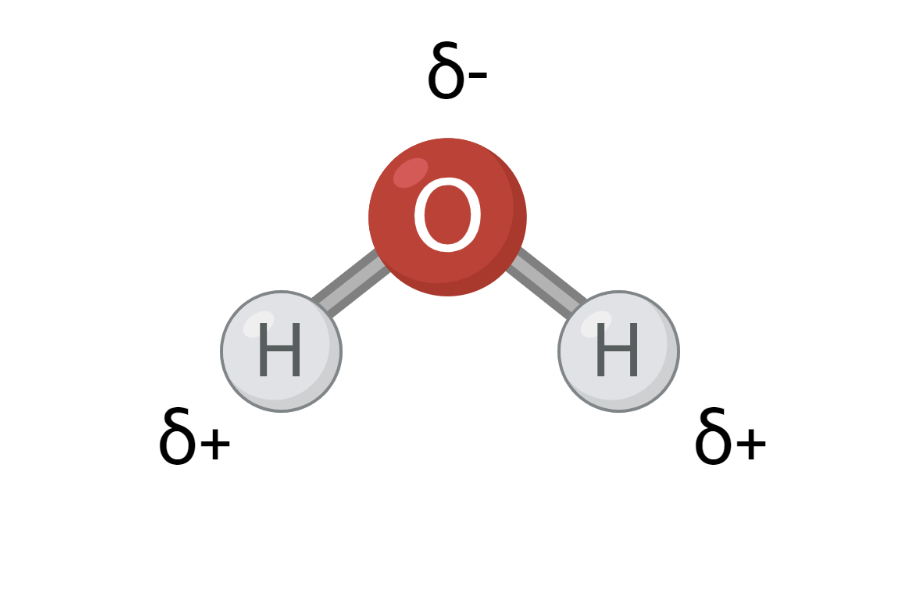
\includegraphics[width=3.25in]{water_polar.png}
\caption{}
\label{fig:water_polar}
\end{wrapfigure}

Whether electrons are shared evenly or unevenly is based on the elements' relative 
\textit{electronegativities}.\index{electronegativity} Electronegativity is simply
a measure of how strongly an atom can attract electrons to itself. In general, 
elements on the right side of the periodic table are more electronegative than 
elements on the left side. When covalent bonds form between two elements of similar electronegativities, the electrons are shared evenly. We call this a \textit{non-polar}
covalent bond. Oil is an example of a non-polar covalent substance. Different 
oils have different ratios and structures, but all oils are made mainly of carbon 
and hydrogen, which have similar electronegativities. What happens when you try to 
mix oil and water? They do not mix well! This is due to the difference between 
their bond types. Polar substances, like water, mix best with other polar 
substances, while non-polar substances, like oils, mix best with non-polar 
substances. You will learn more about why this is in Sequence 2.

For both polar and non-polar covalent bonds, the electrons are held tightly to 
the nuclei, even if they are shared among atoms. Those electrons do not move to 
another molecule: they move around within the molecule they are already a part 
of. Since electrons do not flow freely in covalent substances, they are also poor 
conductors of electricity. Covalent compounds also tend to have lower melting and 
boiling points compared to ionic compounds. 

\subsubsection{Ionic Compounds}
\begin{wrapfigure}{l}{3in}
\noindent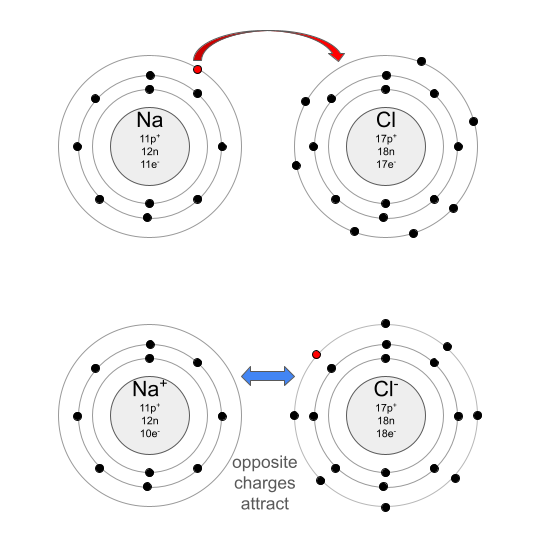
\includegraphics[width=3in]{NaCl_xfer.png}
\caption{}
\label{fig:NaCl_xfer}
\end{wrapfigure}
Ionic bonds are the electrical attraction between opposite-charged ions. When a 
neutral atom gains or loses an electron it becomes an \textit{ion} (a charged 
atom), and oppositely-charged ions are attracted to each other. Which atom gets 
the electron and which loses it is based on their electronegativities: the more 
electronegative atom steals one or more electrons from the less electronegative 
atom.  

Let us examine how a simple ionic compound is formed: sodium chloride, also known 
as table salt, is made up of sodium and chlorine atoms (see figure 
\ref{fig:NaCl_xfer}). When sodium and chlorine come in contact with each other, 
electrons move from the sodium to the chlorine, making a sodium \textit{cation} 
(positively-charged ion) and a chloride \textit{anion} (negatively-charged ion). 
Yes --- chlor\textit{ide} is correct! When naming an anion, the ending of the 
element name changes to \textit{-ide}. Once the sodium cation and chloride anion 
are formed, their opposite charges attract them to each other, like north and 
south magnet poles. 

\begin{wrapfigure}{l}{2in}
\noindent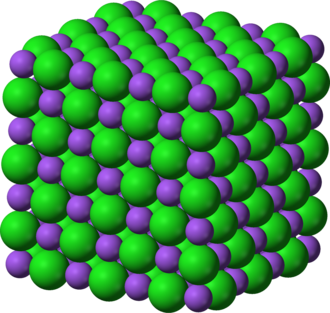
\includegraphics[width=2in]{NaCl_lattice.png}
\caption{}
\label{fig:NaCl_lattice}
\end{wrapfigure} %This figure has issues if it is near the bottom of the page. See Issue #60

When there are many, many sodium and chloride ions around, they spontaneously 
arrange themselves in a pattern, giving ionic compounds their characteristic 
crystal structure (see figure \ref{fig:NaCl_lattice}). Because the electrons are 
tightly held by each ion, ionic substances do not conduct electricity well as 
solids. The atomic crystal lattice also determines the shape of the macroscopic 
crystals. Salt crystals are generally cubic, while other crystals (like quartz) 
form hexagonal prisms. You will learn how to predict the atomic and macroscopic 
crystal structure of different compounds in Sequence 2. 

\subsubsection{Modeling Ionic Compounds}
You can represent ions with Lewis dot diagrams by adding or subtracting electrons 
from the model. Since electrons are negative, anions have gained electrons while 
cations have lost them. Additionally, the ion is in brackets and the overall 
charge is indicated outside the top right corner of the brackets. 

\textbf{Example}: Create Lewis dot diagrams for $\text{Na}^{+}$, $\text{F}^{-}$, 
$\text{O}^{2-}$, and $\text{Mg}^{2+}$.
%FIXME Need more introduction to Lewis dot diagrams.

\textbf{Solution}: Sodium is in column 1, so a neutral sodium atom has 1 valence 
electron. A +1 charge means it has lost 1 electron, leaving zero.
%FIXME "valence electron" has not been defined earlier--needs some introduction.

\begin{center}
    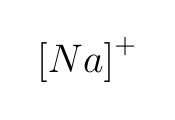
\begin{tikzpicture}
        \node[font = \Large] at (0,0) {$\left[ \text{Na} \right]^{+}$};
     \end{tikzpicture}
\end{center}

Fluorine is in column 17 and has 7 valence electrons when neutral. The anion 
$\text{F}^-$ has gained one electron, for a total of 8. 

\begin{center}
    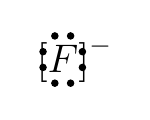
\begin{tikzpicture}
        \node[font = \Large] at (0,0) {$\left[ \text{ F } \right]^-$};
        \draw[fill=black] (-0.4, 0.1) circle (0.4mm);
        \draw[fill=black] (-0.4, -0.1) circle (0.4mm);
        \draw[fill=black] (0.1, 0.1) circle (0.4mm);
        \draw[fill=black] (0.1, -0.1) circle (0.4mm);
        \draw[fill=black] (-0.05, 0.3) circle (0.4mm);
        \draw[fill=black] (-0.25, 0.3) circle (0.4mm);
        \draw[fill=black] (-0.05, -0.3) circle (0.4mm);
        \draw[fill=black] (-0.25, -0.3) circle (0.4mm);
    \end{tikzpicture}
\end{center}

Neutral oxygen has 6 valence electrons. $\text{O}^{2-}$ has gained two, for a full set of 8. 
\begin{center}
    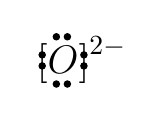
\begin{tikzpicture}
        \node[font = \Large] at (0,0) {$\left[ \text{ O } \right]^{2-}$};
        \draw[fill=black] (-0.5, 0.07) circle (0.4mm);
        \draw[fill=black] (-0.5, -0.07) circle (0.4mm);
        \draw[fill=black] (0.03, 0.07) circle (0.4mm);
        \draw[fill=black] (0.03, -0.07) circle (0.4mm);
        \draw[fill=black] (-0.32, 0.3) circle (0.4mm);
        \draw[fill=black] (-0.18, 0.3) circle (0.4mm);
        \draw[fill=black] (-0.32, -0.3) circle (0.4mm);
        \draw[fill=black] (-0.18, -0.3) circle (0.4mm);
    \end{tikzpicture}
\end{center}

Neutral magnesium has 2 valence electrons. $\text{Mg}^{2+}$ has lost both, leaving none. 
\begin{center}
    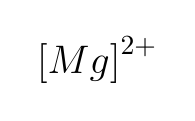
\begin{tikzpicture}
        \node[font = \Large] at (0,0) {$\left[ \text{ Mg } \right]^{2+}$};
    \end{tikzpicture}
\end{center}

Notice the pattern: atoms tend to gain or lose electrons until they have a full outer shell (8) or an empty one.

To make Lewis dot diagrams of ionic compounds, you show both ions in the ratio 
given in the formula. For example, a Lewis dot diagram of $\text{MgCl}_2$ would 
show one magnesium cation and two chloride anions. 

\subsubsection{Metallic Compounds}
You may already know that metals are excellent conductors 
of electricity and heat. This is a consequence of their metallic bonds. In pure 
metals and alloys, the outermost layer of electrons can move freely from one atom 
to the next. As a result, at the atomic level, metals are best characterized as a 
lattice of cations surrounded by a ''sea of electrons" .

The free-flowing sea of electrons in pure and alloyed metal means the cation 
lattice can be rearranged without breaking the metallic bond. As a result, metals 
are ductile (able to be drawn out into a wire) and malleable (able to be hammered 
into a new shape without cracking or breaking). A paperclip bends; a salt crystal shatters.

Metals can be pure, like copper or iron, or \textit{alloys}, like bronze or steel. 
\textit{Alloys} are mixtures between two or more elements where at least one 
element is a metal.\index{alloy} Steel is an alloy of iron and carbon; bronze is 
an alloy of copper and tin. Alloying changes a metal's properties because the different-sized atoms jam the lattice, making it harder for layers to slide. That is why steel is much stronger than pure iron. 

\subsection{Energy and Work}
Look around you: things are moving, warming up, lighting up, and changing. Every one of those changes involves energy moving from one place to another. When a force moves something and transfers energy to it, we say the force does \newterm{work}\index{work}. (No, not the kind you get paid for.) When you climb a flight of stairs, you feel tired. That tiredness is evidence that energy has left your body and gone somewhere else—into lifting your body upward. When the Sun warms your skin, energy is traveling through space and into you. When a moving car comes to a stop, its motion does not simply disappear; energy is transferred to the brakes and the surrounding air, mostly as heat.

Energy Transformations are all around us:
\begin{enumerate}
\item Feeling less tired after consuming calories from food
\item The light and the warmth of the Sun
\item A ball speeding up while rolling down a hill
\item Being out of breath after climbing 5 flights of stairs
\item A car stopping when brakes are applied
\end{enumerate}

Some types of energy are easy to visualize, while others are not. Energy is what  moves from one object to another when work is being done.
There are two main types of energy: energy that is \emph{stored} and energy of motion. Most times, energy that is stored is transformed into energy in motion. This stored energy is called \newterm{Potential Energy}\index{potential energy} and the energy in motion is referred to as \newterm{Kinetic Energy}\index{kinetic energy}. 

When you lift something, the energy stored in your body (in the form of sugar and fat) is 
transferred to the object, accelerating it upwards. Your body continues to 
transfer energy as you lift the object against gravity. When you have lifted it as high as you can, most of the energy your body lost (we call this ``burning Calories'' colloquially) is stored as \textit{Potential Energy}, due to the object's height. Potential energy is the stored energy an object has due to its position or configuration, rather than its motion. \textit{Kinetic Energy} is the term we use to describe the energy an object possesses due to its motion; you will learn more about energy in Section~\ref{chap:conservationMassEnergy}.

Another example of energy is a simple circuit connecting a battery and a light bulb. The battery has stored potential energy. When the circuit is complete, the potential energy in the battery is transferred to electrons in the light bulb, causing them to move and gain kinetic energy. In the light bulb's filament (we are referencing old, non-LED light bulbs here!), the electrons encounter resistance, which slows them down. The energy the electrons lose in this process is being transformed into 
light and heat, lighting your room. 

The work-energy theorem, from the Work and Energy chapter, makes the link between work and energy exact. 

\subsection{Mass-Energy Equivalence}
You have probably seen the equation
$$E = mc^2$$

$E$ is energy, $m$ is mass, and $c$ is the speed of light in a vacuum (about $3 
\times 10^8 \frac{m}{s}$). So far, we have been discussing matter and energy 
separately. This equation shows that matter can be converted to energy, and
vice-versa.\index{mass-energy equivalence} This is the source of the light energy emitted by the sun. 

The Sun is mostly hydrogen. At the very center, it is so hot and dense that the 
nuclei of hydrogen atoms are fused together to form helium atoms, a process 
called the \textit{proton-proton chain reaction}. The actual reaction involves several 
steps and is more complicated, but the overall process can be summarized as:

$$4\text{H} \to \text{He}$$

If every hydrogen atom has a mass of approximately $1.6735575 \times 10^{-27}$ kg 
and every helium atom has a mass of approximately $6.6464731 \times 10^{-27}$ kg, 
how much energy is released when one atom of helium is created? First, notice 
that one helium has less mass than 4 hydrogen atoms:

$$4 \times \left( 1.6735575 \times 10^{-27} \right) - 6.6464731 \times 10^{-27} = 
4.77569 \times 10^{-29}$$

Now, we can use $E = mc^2$ to find out how much energy is equivalent to $4.77569 
\times 10^{-29}$ kg:

$$E = \left( 4.77569 \times 10^{-29} \text{kg} \right) \left( 2.99792458 \times 
10^8 \frac{\text{m}}{\text{s}} \right)^2$$
$$E \approx 4.292 \times 10^{-12} \text{joules}$$

That is a tiny number, so let us scale up. Suppose you fused 1 kilogram of hydrogen (as a gas, enough to fill a small bedroom). The lost mass is $\frac{4.77569 \times 10^{-29}}{4 \times 1.6735575 \times 10^{-27}} \approx 0.71\%$ of the hydrogen's mass, so about 0.00713 kg disappears, roughly the mass of three pennies.

$$E = \left( 0.00713 \text{ kg} \right) \left( 2.99792458 \times 10^8 \frac{
\text{m}}{\text{s}} \right)^2 \approx 6.4 \times 10^{14} \text{ joules}$$

That is about 180,000,000 kWh (kilowatt-hours). An average US home uses about 30 kWh per day, so one kilogram of hydrogen could power a home for \textit{over 16,000 years}! That is why scientists keep working on nuclear fusion power. The nuclear power plants currently running around the world 
today rely on \textit{nuclear fission}\index{nuclear fission}: the splitting apart of atoms, the opposite
process of \textit{nuclear fusion}.\index{nuclear fusion} Fission releases several times less energy 
per kilogram of fuel than fusion, and thus stable, affordable 
nuclear fusion power plants remain a ''holy grail" of scientific research. 

\subsection{Conclusion}
We have seen that the universe is made of dark energy, dark matter, and ordinary matter. Ordinary matter is made of atoms, which can be classified based on their number of protons. Atoms combine in different ways to make compounds, and the manner of combination (ionic, covalent, or metallic bonding) affects the macroscopic properties of the substance. Energy allows matter to do work, and work is the transfer of energy. 

Matter and energy share one more property: neither can come from nothing or vanish into nothing.\index{conservation of mass and energy} As you just saw, $E = mc^2$ lets a little mass turn into a lot of energy, but the total of the two never changes. In chemistry and everyday life, the mass that turns into energy is far too small to measure, so we can treat mass and energy as each conserved on its own. That idea is the subject of the next section.







%FIXME Global layout note: Let's discuss adding Titles and Captions to all graphics.\\

%For example:\\
%TITLE: Mass versus Weight\\
%CAPTION: Human Earth weight: 150lbs / Moon weight:??lbs\\
%Potato Earth weight: .25lbs / Moon weight: ??lbs \\

%FIXME:
%Allison thinks it would be funny if the person in the graphic were holding a potato and we also added the weight and mass of the potato to the caption. No worries if this type of edit isn't in the budget!

%FIXME: What are your thoughts about using the metric system consistently -- in which case we'll replace pounds here with kilos. Max notes: we should explicitly use kilos for mass and pounds or newtons for weight. Kilos are a scalar measure of the amount of matter and pounds are a vector force of gravity on a particular piece of matter. Many students struggle to differentiate between mass and weight at a theoretical level due to casual comparison between pounds and kilos.


\section{Conservation of Mass and Energy}\label{chap:conservationMassEnergy}
One of the most powerful laws in science says that mass and energy\index{conservation of mass and energy} cannot be created or destroyed, only moved around or changed in form. 

\subsection{Conservation of Mass}
Since matter cannot be created or destroyed, a chemical reaction does not change 
the mass of the \textit{reactants}\index{reactants} as they form \textit{products}\index{products}. Consider the reaction between 
vinegar and baking soda, which produces carbon dioxide, water, and sodium acetate:

\begin{center}
    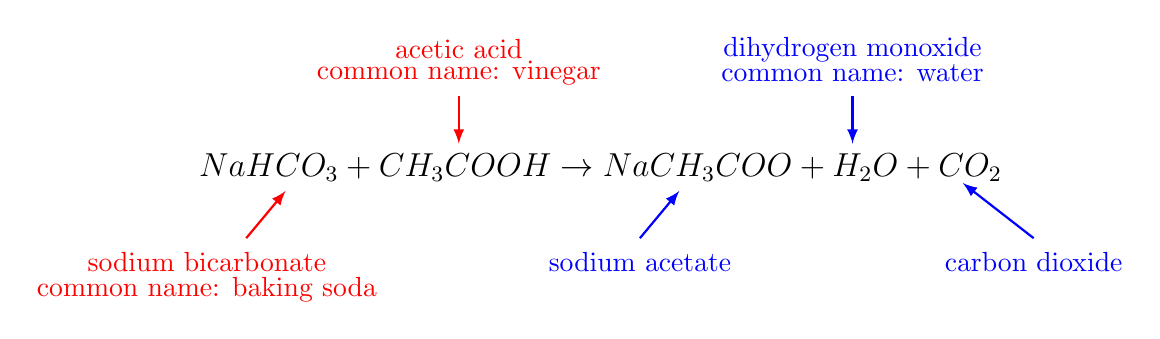
\begin{tikzpicture}
        \node[font = \large] at (0,0) {$NaHCO_3 + CH_3COOH \to NaCH_3COO + H_2O + CO_2$};
        \node[red] at (-5, -1.2) {sodium bicarbonate};
        \node[red] at (-5, -1.55) {common name: baking soda};
        \draw[thick, red, -latex] (-4.5, -0.9) -- (-4, -0.3);
        \node[red] at (-1.8, 1.2) {common name: vinegar};
        \node[red] at (-1.8, 1.5) {acetic acid};
        \draw[thick, red, -latex] (-1.8, 0.9) -- (-1.8, 0.3);
        \node[blue] at (0.5, -1.2) {sodium acetate};
        \draw[thick, blue, -latex] (0.5, -0.9) -- (1, -0.3);
        \node[blue] at (3.2, 1.5) {dihydrogen monoxide};
        \node[blue] at (3.2, 1.2) {common name: water};
        \draw[thick, blue, -latex] (3.2, 0.9) -- (3.2, 0.3);
        \node[blue] at (5.5, -1.2) {carbon dioxide};
        \draw[thick, blue, -latex] (5.5, -0.9) -- (4.6, -0.2);
    \end{tikzpicture}
\end{center}

The reactants are labeled with red, and the products with blue. This equation is
\textit{balanced}: that is, it shows the same number of each element on each side
of the arrow. This shows that the atoms are not created or destroyed during a 
chemical reaction, they are only rearranged. Take a minute to count up each 
element on each side. You should find there are 5 hydrogens, 1 sodium, 3 carbons,
and 5 oxygens on each side. 

Now, let us look at an \textit{unbalanced} chemical reaction. As you know, hydrogen
and oxygen combine to form water. Additionally, hydrogen and oxygen both exist as
\textit{diatomic gases}\index{diatomic molecules}. When we say "oxygen gas" or "hydrogen gas", we mean the 
diatomic molecules, $O_2$ and $H_2$, respectively. Here is an unbalanced chemical 
reaction between hydrogen gas and oxygen gas to form water:

\begin{center}
    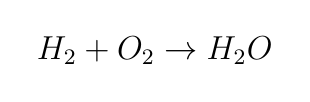
\begin{tikzpicture}
        \node[font = \large] at (0,0) {$H_2 + O_2 \to H_2O$};
    \end{tikzpicture}
\end{center}

How do we know this equation is unbalanced? Count up the elements: there are two 
oxygen atoms on the reactant side, but only one on the product side. This violates 
the conservation of matter: that oxygen atom cannot just disappear!

\subsubsection{Balancing Chemical Reactions}
We solve this by \textit{balancing}\index{balancing chemical reactions} the chemical reaction: adjusting the number 
of products and reactants to comply with the Law of Conservation of Matter. You will
learn strategies for balancing chemical reactions in Sequence 2, but for now we will
briefly balance this chemical reaction so that it complies with the Law of 
Conservation of Matter. You may be tempted to simply add a lone oxygen atom to 
the products side:

\begin{center}
    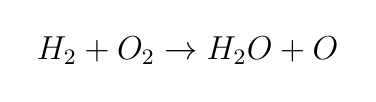
\begin{tikzpicture}
        \node[font = \large] at (0,0) {$H_2 + O_2 \to H_2O + O$};
    \end{tikzpicture}
\end{center}

The major reason this is incorrect is that oxygen does not exist as a lone atom -
as discussed above - so it does not make sense to have a lone oxygen as a product. 
So maybe we should add a molecule of oxygen gas to both sides?

\begin{center}
    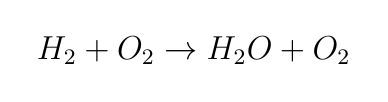
\begin{tikzpicture}
        \node[font = \large] at (0,0) {$H_2 + O_2 \to H_2O +O_2$};
    \end{tikzpicture}
\end{center}

Well, now we have the same problem we started with: the oxygens are unbalanced. 
When balancing chemical reactions, we can only add \textit{whole molecules} that 
are already in the reaction. Let us take another look at our unbalanced reaction 
with some molecular models for visualization:

\begin{center}
    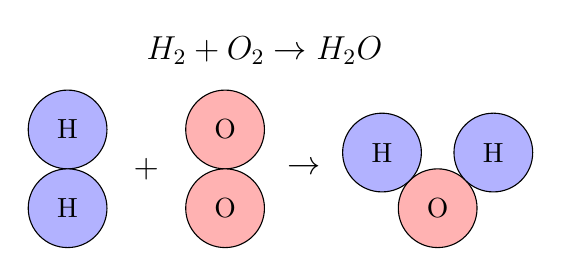
\begin{tikzpicture}
        \node[font = \large] at (0,0) {$H_2 + O_2 \to H_2O$};
        \draw[draw=black, fill=blue!30] (-2.5, -1) circle (0.5);
        \draw[draw=black, fill=blue!30] (-2.5, -2) circle (0.5);
        \node[] at (-2.5, -1) {H};
        \node[] at (-2.5, -2) {H};
        \node[font = \large] at (-1.5, -1.5) {+};
        \draw[draw=black, fill=red!30] (-0.5, -1) circle (0.5);
        \draw[draw=black, fill=red!30] (-0.5, -2) circle (0.5);
        \node[] at (-0.5, -1) {O};
        \node[] at (-0.5, -2) {O};
        \node[font = \large] at (0.5, -1.5) {$\to$}; 
        \draw[draw=black, fill=red!30] (2.2, -2) circle (0.5);
        \node[] at (2.2, -2) {O};
        \draw[draw=black, fill=blue!30] (1.493, -1.293) circle (0.5);
        \draw[draw=black, fill=blue!30] (2.907, -1.293) circle (0.5);
        \node[] at (1.493, -1.293) {H};
        \node[] at (2.907, -1.293) {H};
    \end{tikzpicture}
\end{center}

You can clearly see we need more oxygens on the product side. Since we can only 
add \textit{whole molecules}, our only option is to add another water. We do this
by adding a coefficient of 2 in front of $H_2O$ in our equation, which indicates 
2 water molecules (just like $2x$ means two x's):

\begin{center}
    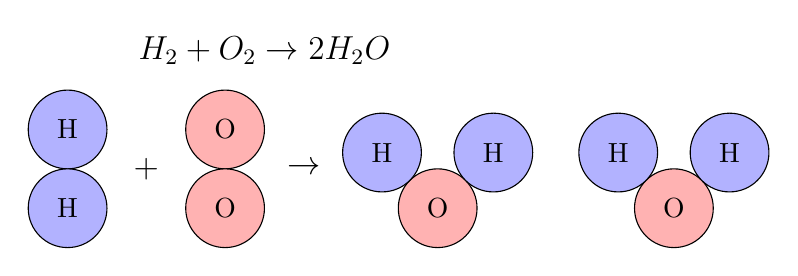
\begin{tikzpicture}
        \node[font = \large] at (0,0) {$H_2 + O_2 \to 2H_2O$};
        \draw[draw=black, fill=blue!30] (-2.5, -1) circle (0.5);
        \draw[draw=black, fill=blue!30] (-2.5, -2) circle (0.5);
        \node[] at (-2.5, -1) {H};
        \node[] at (-2.5, -2) {H};
        \node[font = \large] at (-1.5, -1.5) {+};
        \draw[draw=black, fill=red!30] (-0.5, -1) circle (0.5);
        \draw[draw=black, fill=red!30] (-0.5, -2) circle (0.5);
        \node[] at (-0.5, -1) {O};
        \node[] at (-0.5, -2) {O};
        \node[font = \large] at (0.5, -1.5) {$\to$}; 
        \draw[draw=black, fill=red!30] (2.2, -2) circle (0.5);
        \node[] at (2.2, -2) {O};
        \draw[draw=black, fill=blue!30] (1.493, -1.293) circle (0.5);
        \draw[draw=black, fill=blue!30] (2.907, -1.293) circle (0.5);
        \node[] at (1.493, -1.293) {H};
        \node[] at (2.907, -1.293) {H};

        \draw[draw=black, fill=red!30] (5.2, -2) circle (0.5);
        \node[] at (5.2, -2) {O};
        \draw[draw=black, fill=blue!30] (4.493, -1.293) circle (0.5);
        \draw[draw=black, fill=blue!30] (5.907, -1.293) circle (0.5);
        \node[] at (4.493, -1.293) {H};
        \node[] at (5.907, -1.293) {H};
    \end{tikzpicture}
\end{center}

We have fixed our oxygen problem: now there are two oxygen atoms on both sides. 
But now we have a hydrogen problem: there are 2 on the reactant side and 4 on 
the product side. We can address this by adding another hydrogen gas molecule 
to the reactant side:

\begin{center}
    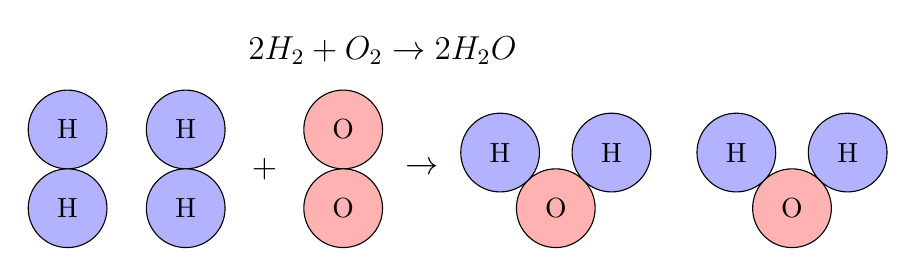
\begin{tikzpicture}
        \node[font = \large] at (0,0) {$2H_2 + O_2 \to 2H_2O$};
        \draw[draw=black, fill=blue!30] (-4, -1) circle (0.5);
        \draw[draw=black, fill=blue!30] (-4, -2) circle (0.5);
        \node[] at (-4, -1) {H};
        \node[] at (-4, -2) {H};
        
        \draw[draw=black, fill=blue!30] (-2.5, -1) circle (0.5);
        \draw[draw=black, fill=blue!30] (-2.5, -2) circle (0.5);
        \node[] at (-2.5, -1) {H};
        \node[] at (-2.5, -2) {H};
        \node[font = \large] at (-1.5, -1.5) {+};
        \draw[draw=black, fill=red!30] (-0.5, -1) circle (0.5);
        \draw[draw=black, fill=red!30] (-0.5, -2) circle (0.5);
        \node[] at (-0.5, -1) {O};
        \node[] at (-0.5, -2) {O};
        \node[font = \large] at (0.5, -1.5) {$\to$}; 
        \draw[draw=black, fill=red!30] (2.2, -2) circle (0.5);
        \node[] at (2.2, -2) {O};
        \draw[draw=black, fill=blue!30] (1.493, -1.293) circle (0.5);
        \draw[draw=black, fill=blue!30] (2.907, -1.293) circle (0.5);
        \node[] at (1.493, -1.293) {H};
        \node[] at (2.907, -1.293) {H};

        \draw[draw=black, fill=red!30] (5.2, -2) circle (0.5);
        \node[] at (5.2, -2) {O};
        \draw[draw=black, fill=blue!30] (4.493, -1.293) circle (0.5);
        \draw[draw=black, fill=blue!30] (5.907, -1.293) circle (0.5);
        \node[] at (4.493, -1.293) {H};
        \node[] at (5.907, -1.293) {H};
    \end{tikzpicture}
\end{center}

And now we have the same number of hydrogens and oxygens on each side! Notice we 
have all the same reactants and products that we started with, but now in ratios 
that reflect the conservation of matter. 

A final note: if atoms are in parentheses followed by a subscript, the subscript 
applies to every atom in the parentheses. For example, zinc nitrate, $Zn \left( 
NO_3 \right)_2$ is made of 1 zinc, 2 nitrogens, and 6 oxygens. 

\begin{Exercise}[title = {Balanced and Unbalanced Reactions}, label = balance]
Classify the following chemical reactions as balanced or unbalanced. If it is 
unbalanced, state what element(s) are not conserved. 
\begin{enumerate}
\item $NiCl_2 + 2NaOH \to Ni \left(OH \right)_2 + 2NaCl$
\item $HgO \to Hg + O_2$
\item $BaSO_4 + 2C \to 2BaS + CO$
\item $Cd \left( NO_3 \right)_2 + H_2S \to CdS + 2HNO_3$
\end{enumerate}
\end{Exercise}

\begin{Answer}[ref = balance]
\begin{enumerate}
\item balanced
\item unbalanced; oxygen
\item unbalanced; barium, sulfur, oxygen, and carbon
\item balanced
\end{enumerate}
\end{Answer}

\subsection{Conservation of Energy in Systems}
Just like matter, energy is also conserved\index{conservation of energy}: it cannot be created or destroyed, 
only change forms. You met the main types of energy in the Work and Energy chapter. The transformation of energy from one type to another 
drives our modern world: your phone transforms electrical potential energy into 
light and sound energy, a nuclear power plant transforms nuclear energy to 
electrical energy, and your car transforms chemical potential energy (in the 
gasoline) into kinetic energy (motion).

\subsubsection{Friction, Heat, and Energy "Loss"}
Imagine rolling a ball across a flat surface: you have given the ball some 
kinetic energy in its motion. If the kinetic energy were conserved, the ball 
would keep rolling at the same speed forever, as long as it was on a flat 
surface. Experience tells us this is not what happens: the ball will eventually 
come to a stop. Why does this not violate the conservation of energy?

Friction\index{friction} is the force that opposes motion: whenever you slide two objects past 
each other, friction transforms kinetic energy into heat. Rub the palms of your 
hands together. You should feel warmth, a product of the friction between your 
hands. As the ball in the example above rolls, it also experiences friction 
between itself and the ground. The friction slowly transforms the kinetic energy 
of the ball into heat, causing the ball to lose kinetic energy. When all of the 
ball's kinetic energy is transformed to heat, the ball comes to a rest. So, the 
kinetic energy of the ball was not destroyed and did not disappear: it became heat. 

In fact, nearly all energy in the universe will eventually be transformed to heat,
resulting in the inevitable "heat death"\index{heat death of the universe} of the universe. Here is a short video 
about heat, entropy, and the heat death of the universe: 
\url{https://www.youtube.com/watch?v=gOWt_Hq3yrE/}. 

\subsubsection{Energy Conservation in Falling Objects}
When an object is positioned above the ground, it has \textit{gravitational 
potential energy}\index{gravitational potential energy}\index{potential energy}. 
The potential energy is proportional to the mass of the object, the strength of 
the gravitational field, and the object's height above the ground:

$$E_{p} = mgh$$

where $m$ is the mass of the object in kg, $g$ is the acceleration due to gravity 
($9.8 m/s^2$ on Earth), and $h$ is the height above the ground in meters. 

\textbf{Example}: What is the gravitational potential energy of a 5.0 kilogram 
bowling ball in the hand of a bowler (approximately 1.2 meters high)?

\textbf{Solution}: The mass is 5.0 kg, the height is 1.2 m, and we assume the 
bowler is on Earth, so g is 9.8 $m/s^2$:

$$E_{p} = \left( 5.0 kg \right) \left( 9.8 m/s^2 \right) \left( 1.2 m \right) = 59 J$$

Here is a new unit: \textit{joules}\index{joule}, represented by a capital J. A joule is a 
unit of energy, and it is the same as $\frac{kg \cdot m^2}{s^2}$. 

If the bowler were to drop that ball, it would lose potential energy and gain 
\textit{kinetic energy}\index{kinetic energy}. The kinetic energy of an object 
is proportional to its mass and the square of its speed:

$$E_{k} = \frac{1}{2}mv^2$$

where mass is in kg and speed (v) is in m/s. You can quickly check that the units 
still come out to a joule! If there is no air resistance, then as an object falls 
all of its potential energy is converted to kinetic energy. (If you'd like to 
explore what happens when friction is accounted for, you can play with this PhET 
simulation: \url{https://phet.colorado.edu/en/simulations/energy-skate-park}.)

\textbf{Example}: If the bowling ball were dropped, what would its speed be right 
before it hits the ground? (Neglect air resistance.)

\textbf{Solution}: Ignoring air resistance, according to the Law of Conservation 
of Energy, the kinetic energy of the ball right before it hits the ground must be 
equal to the gravitational potential energy of the ball right before its release. 
Therefore:

$$mgh = \frac{1}{2}mv^2$$

We can eliminate an $m$ from both sides and rearrange to solve for $v$:

$$v = \sqrt{2gh} = \sqrt{2 \left( 9.8 m/s^2 \right) \left(1.2 m \right)} = 
\sqrt{23.52 \frac{m^2}{s^2}} = 4.8 \frac{m}{s}$$

The ball will have a speed of 4.8 m/s just before it hits the ground. 

\begin{Exercise}[title = {Kinetic and Potential Energy}, label = ke_pe]
\begin{enumerate}
\item How fast should you toss a ball straight up if you want it to reach your 
friend on the second floor (3.7 meters above you)?
\item Your little brother is teasing you from a treehouse 5.0 meters off the 
ground. If your slingshot can shoot a pebble at 15 m/s, can you hit your little 
brother?
\item A 63-kg roller-blader rolls down a hill. If the hill is 8.0 meters high and 
she reaches the bottom of the hill with a speed of 11.2 m/s, how much energy was 
converted to heat through friction?
\end{enumerate}
\vspace{25mm}
\end{Exercise}

\begin{Answer}[ref = ke_pe]
\begin{enumerate}
\item $v = \sqrt{2gh} = \sqrt{2 \left( 9.8 m/s^2 \right) \left( 3.7 m \right)} = 
8.5 m/s$
\item $h = \frac{v^2}{2g} = \frac{\left( 15 \frac{m}{s} \right)^2}{2 \left( 9.8 
\frac{m}{s^2} \right)} = 11.5 m$. You can hit your little brother, since you could 
shoot the pebble as high as 11.5 m and he is only 5.0 m above you.
\item We know that $E_{p, initial} = E_{k, final} + E_{lost to friction}$. 
Therefore, $E_{lost\_to\_friction} = E_{p, initial} - E_{k, final} = mgh - \frac{1}{2}
mv^2 = \left(63 kg \right) \left( 9.8 \frac{m}{s^2} \right) \left( 8 m \right) -
\frac{1}{2} \left( 63 kg \right) \left( 11.2 \frac{m}{s} \right)^2 = 4939.2 J - 
3951.4 J = 988 J$. 
\end{enumerate}
\end{Answer}

\subsection{Types of Systems}
We classify systems based on the flow of matter and energy. A \textit{system} is 
a set of interconnected elements. Your body is a system, as is a television or a 
boiling pot of water. Scientists define systems by separating the parts of the 
system from the rest of the universe, usually called "the surroundings". You can 
represent this separation with a dashed line. Here is a diagram defining a pot of
boiling water as a system:

\begin{center}
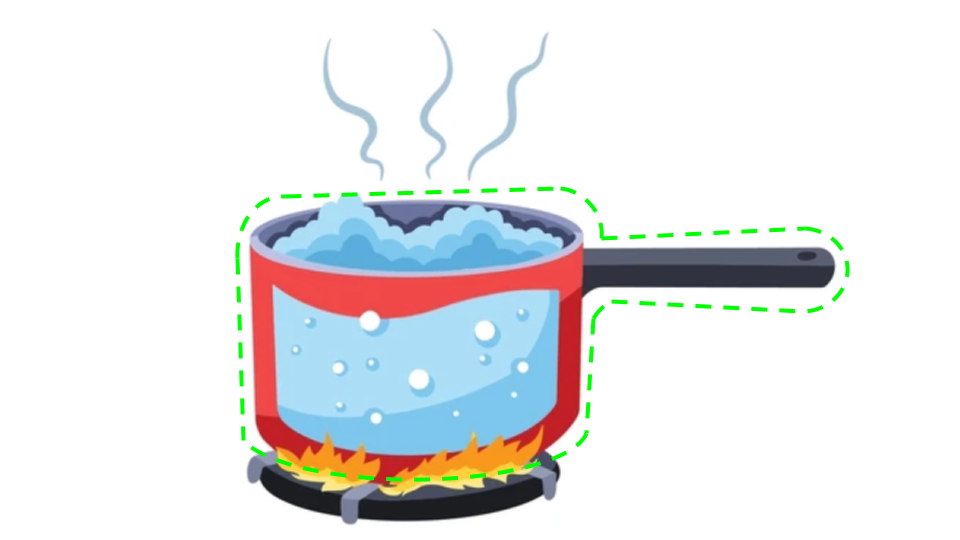
\includegraphics[width=4in]{pot_open_system.png}
\end{center}

Everything inside the dashed line is the system: the pot and the water boiling in
it. Everything outside the dashed line is the surroundings: the stove, the air 
around the pot, etc. Defining a system is \textit{arbitrary}: there is not one hard 
and fast definition of a system. Think of your school: you could look at the 
system of a classroom, the system of a hallway and all the classes connected to 
it, or the entire school building. How you define a system depends on what you are 
studying. 

\subsubsection{Open Systems}
An \textit{open system} allows for matter and energy to cross the imaginary 
boundary between the system and its surroundings. The uncovered pot of boiling 
water is an example of an open system. Energy enters the system as heat from the
stove, and leaves the system as heat in the steam rising from the pot. Notice 
that steam rising: see how it crosses the imaginary boundary? The steam is matter 
\textit{leaving the system}. Since matter and energy can cross the boundary 
between the system and its surroundings, the uncovered boiling pot is an open 
system. \index{open system}

\begin{center}
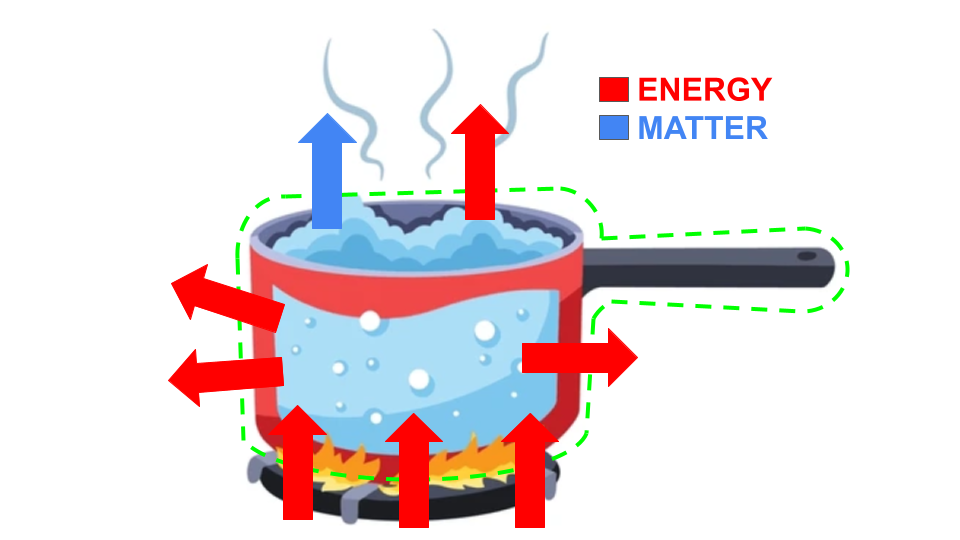
\includegraphics[width=4in]{pot_open_arrows.png}
\end{center}

The system also loses energy through the sides of the pot: if you touched the 
pot, it would feel hot, which means heat energy can also leave the system through
the sides of the pot. This is due to the collision between air particles (the 
surroundings) and the outside of the pot (the system). With every collision, a 
little heat is transferred from the pot to the air. This is why your hot drink 
gets cold if you leave it out, even if you do not add any ice. 

\subsubsection{Closed Systems}
A \textit{closed system} allows for the transfer of energy but not the transfer 
of matter. If we put a lid on this pot, it would become a closed system. 
\index{closed system}

\begin{center}
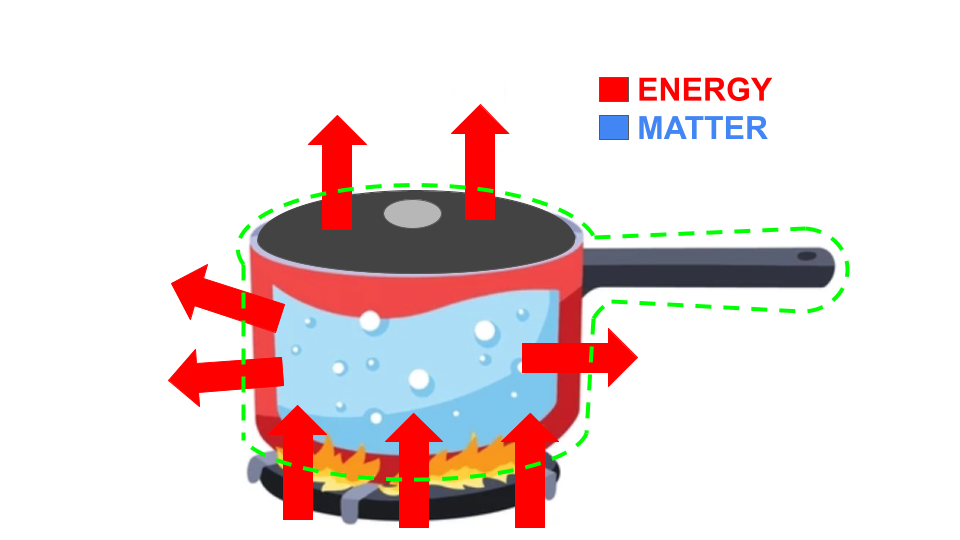
\includegraphics[width=4in]{pot_closed_system.png}
\end{center}

Notice that the difference between an open and closed system is the flow of 
\textit{matter}: open systems allow for the movement of matter, while closed 
systems do not. However, energy can still enter and leave closed systems. 
Sealed containers that are not insulated are good examples of closed systems - 
a car with the windows up and doors closed. 

\subsubsection{Isolated Systems}
An \textit{isolated system}\index{isolated system} does not allow for the flow of matter \textit{or} 
energy in or out of the system. There is no such thing as a truly isolated system: in reality, a small amount of energy can be transferred even through the best 
thermal insulators. However, for well-insulated systems, it can be a good 
approximation to model that system as isolated. A simple example would be a 
sealed, well-insulated coffee thermos. The transfer of heat energy between the 
coffee in the thermos and the thermos' surroundings is so slow that we can ignore
that small amount of transfer and approximate the thermos as an isolated system. 

\subsubsection{Classifying Systems}
To quickly categorize a system as open, closed, or isolated, ask yourself two questions:
\begin{enumerate}
\item Can matter enter or leave the system?
\item Can energy enter or leave the system?
\end{enumerate}

If your answer to the first question is yes, you know automatically the system 
is open. If no, move to the second question. If energy can enter or leave, the 
system is closed. If not, the system is isolated. Sometimes, textbooks and exams 
will describe a system as "well-insulated". This is directing you to assume any 
transfer of energy between the system and surroundings is negligible, and that 
you should treat the system as an isolated system. 

\begin{Exercise}[title = {Open, Closed, and Isolated Systems}, label = systems]
Classify each system as open, closed, or isolated. Justify your answer. 
\begin{enumerate}
\item The human body
\item Earth
\item Your cell phone
\item A well-insulated cooler with the lid sealed
\item A well-insulated cooler with the lid open
\item A bottle of soda before it is opened to be drunk
\end{enumerate}
\end{Exercise}

\begin{Answer}[ref = systems]
\begin{enumerate}
\item The human body is an open system because matter can enter (food, water, 
oxygen) and leave (waste, carbon dioxide, sweat) your body.
\item The Earth is an open system because matter can enter (asteroids falling, 
spaceships returning) and leave (space vehicles and astronauts). On the other 
hand, the Earth can be well-approximated as a closed system. Before the 20th 
Century, humans had no way to deliberately expel matter from the Earth, and the 
mass of asteroids that are pulled in by the Earth's gravity is negligible 
compared to the Earth. Therefore, in the right circumstances, it would be 
appropriate to model the Earth as a closed system. (It is closed because 
energy in the form of sunlight is constantly entering the system.)
\item A cell phone is a closed system - you do not put any matter in or take it 
out of your phone, but it constantly uses battery and then is recharged, showing
that energy enters and leaves your phone. 
\item Since the cooler is described as well-insulated and the lid is closed, it 
can be approximated as an isolated system. Scientific equipment, like bomb 
calorimeters, rely on this approximation. 
\item With the lid open, matter can enter and leave and therefore the cooler is 
an open system (yes, even though it is well-insulated). 
\item A sealed bottle of soda is a closed system - the soda and carbon dioxide 
cannot escape, but energy in the form of heat can be transferred in and out of 
the system (the contents of the bottle will lose heat if you put it in the 
fridge and gain heat if you leave it in the sun).
\end{enumerate}
\end{Answer}
